\documentclass[10pt]{article}
\author{Alex Peyrard}
\title{Digital Image Processing}
\usepackage{graphicx}

\begin{document}
\maketitle
\section{Introduction}
All of the programs are written in python 3. The shebangs are included and thus they should work if called using the "./program.py" notation. In case this causes a problem, please try to call them using "python3 program.py" notation.\\\\
I will provide further help on how to call each program.
\subsection{libraries}
I used numpy in all of the programs and scipy in some of them. I will detail when scipy is used.
\section{Exercise 1}
The program called ex1.py computes the histogram of a greyscale image, and enhances the image using histogram equalization. it displays the enhanced image, the histograms of the default and enhanced images, and the transformation function.\\
In this exercise, the matplotlib library is used to plot hitograms and functions.
\subsection{Examples}
\subsubsection{Fig1.jpg}
All of the results are obtained using the program with the call "./ex1.py Fig1.jpg"
\begin{figure}[!ht]
	\centering
	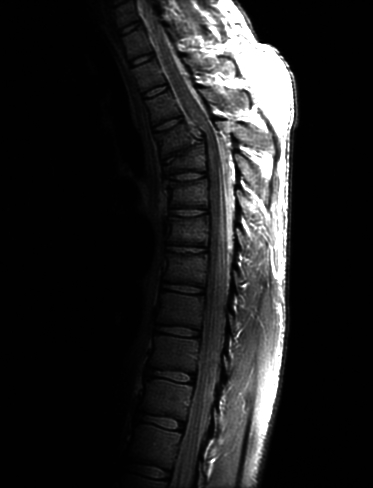
\includegraphics[height=200pt]{./ex1/Fig1.jpg}
	\caption{Original image}
\end{figure}
\begin{figure}[!ht]
	\centering
	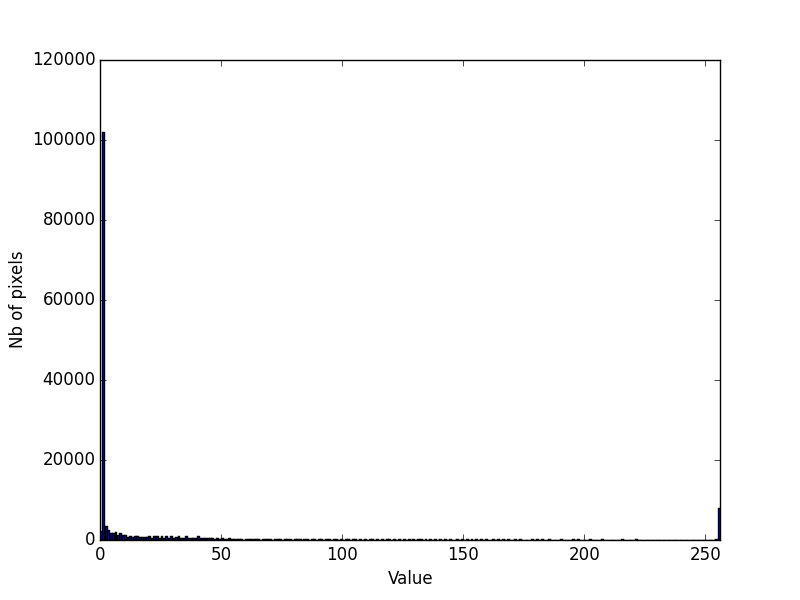
\includegraphics[height=200pt]{./ex1/Fig1_hist.png}
	\caption{Original image's histogram}
\end{figure}
\begin{figure}[!ht]
	\centering
	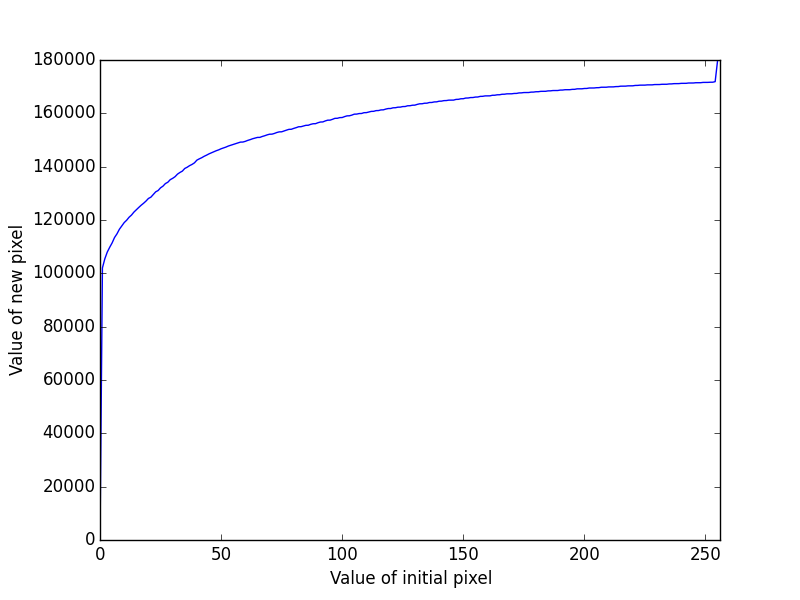
\includegraphics[height=200pt]{./ex1/Fig1_cdf.png}
	\caption{Enhancement function}
\end{figure}
\begin{figure}[!ht]
	\centering
	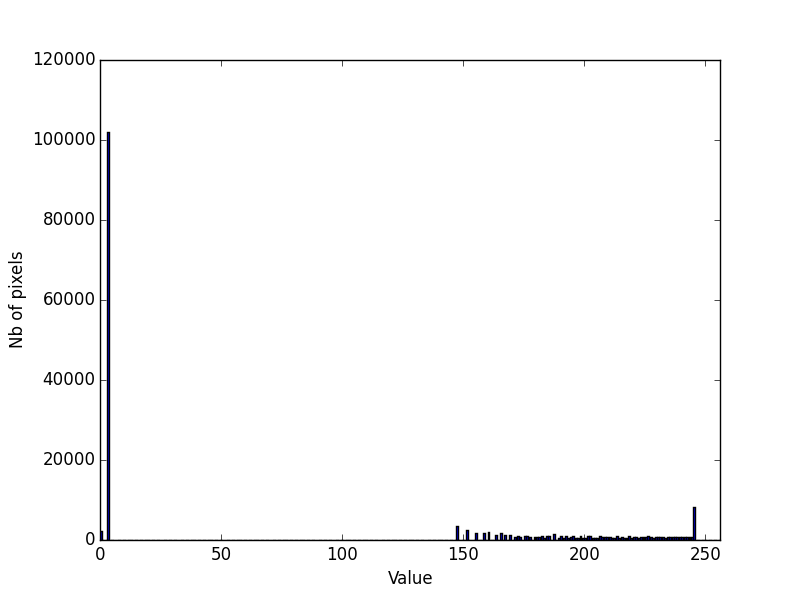
\includegraphics[height=200pt]{./ex1/Fig1_enh_hist.png}
	\caption{Enhanced image histogram}
\end{figure}
\begin{figure}[!ht]
	\centering
	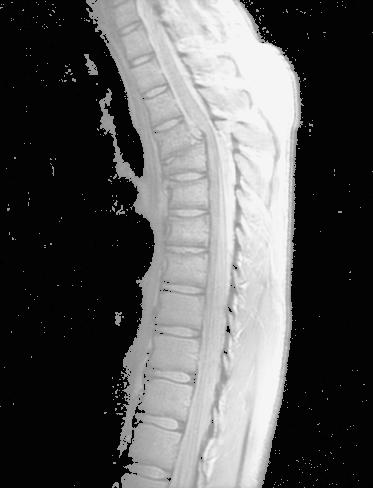
\includegraphics[height=200pt]{./ex1/Fig1_enh.jpg}
	\caption{Enhanced image}
\end{figure}
\clearpage

\subsubsection{Fig2.jpg}
All of the results are obtained using the program with the call "./ex1.py Fig2.jpg"
\begin{figure}[!ht]
	\centering
	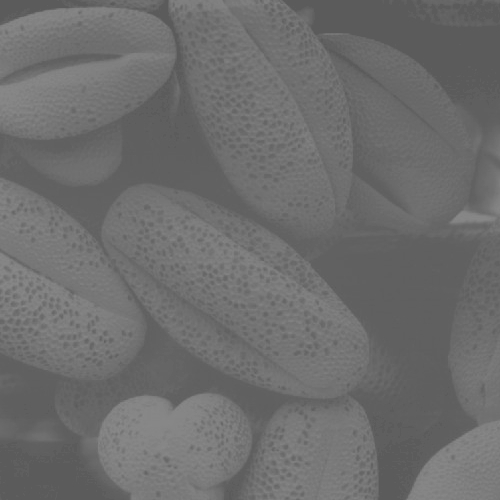
\includegraphics[height=200pt]{./ex1/Fig2.jpg}
	\caption{Original image}
\end{figure}
\begin{figure}[!ht]
	\centering
	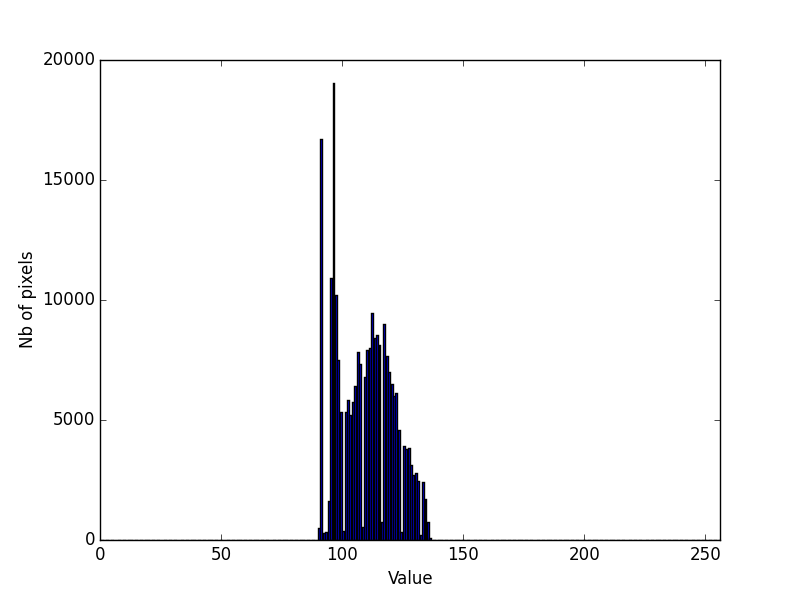
\includegraphics[height=200pt]{./ex1/Fig2_hist.png}
	\caption{Original image's histogram}
\end{figure}
\begin{figure}[!ht]
	\centering
	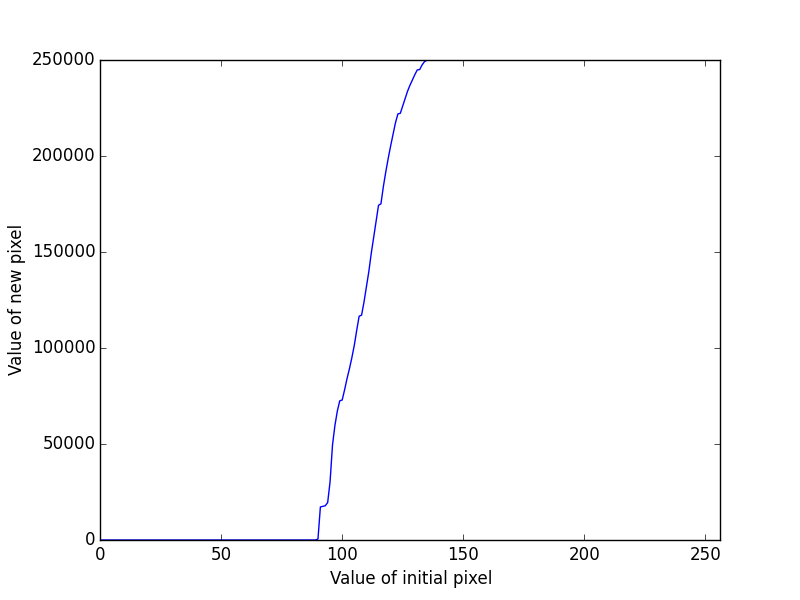
\includegraphics[height=200pt]{./ex1/Fig2_cdf.png}
	\caption{Enhancement function}
\end{figure}
\begin{figure}[!ht]
	\centering
	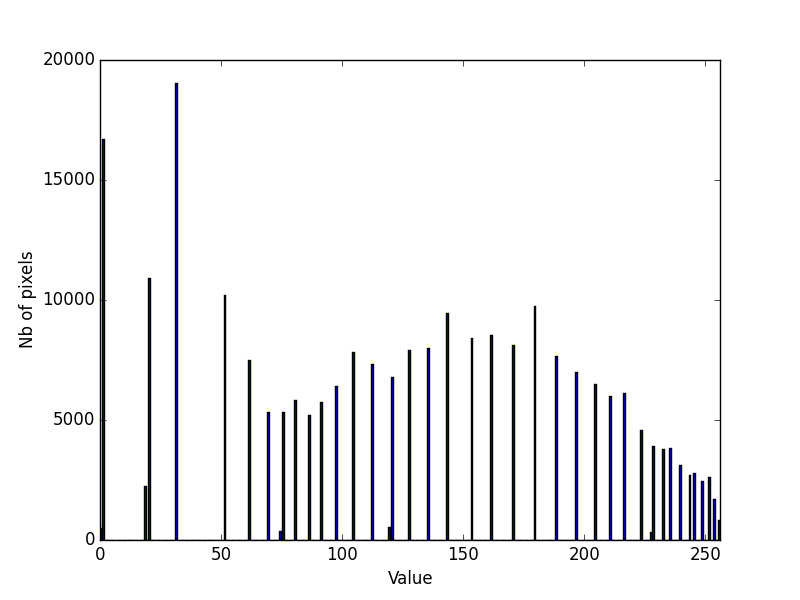
\includegraphics[height=200pt]{./ex1/Fig2_enh_hist.png}
	\caption{Enhanced image histogram}
\end{figure}
\begin{figure}[!ht]
	\centering
	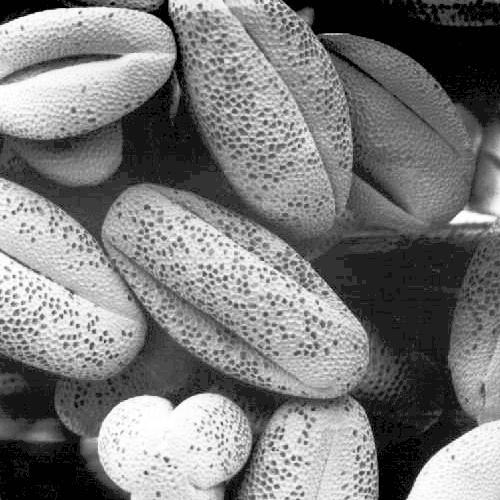
\includegraphics[height=200pt]{./ex1/Fig2_enh.jpg}
	\caption{Enhanced image}
\end{figure}
\clearpage

\section{Exercise 2}
The program called ex2.py performs several spatial enhancement techniques on a given greyscale image.
\subsection{Example on skeleton\_orig.tif}
All of the results are obtained using the program with the call "./ex2.py skeleton\_orig.tif"
\begin{figure}[!ht]
	\centering
	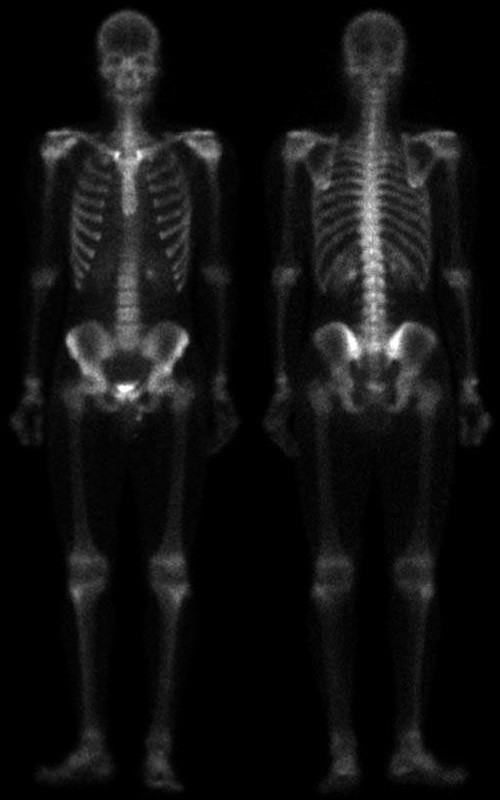
\includegraphics[height=200pt]{./ex2/skeleton_orig.jpg}
	\caption{Original image}
\end{figure}
\begin{figure}[!ht]
	\centering
	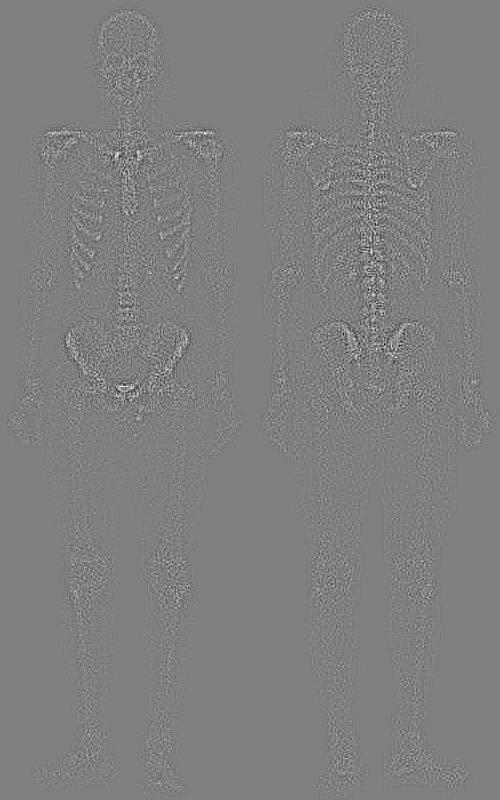
\includegraphics[height=200pt]{./ex2/skeleton_lap.jpg}
	\caption{Rescaled laplacian of image}
\end{figure}
\begin{figure}[!ht]
	\centering
	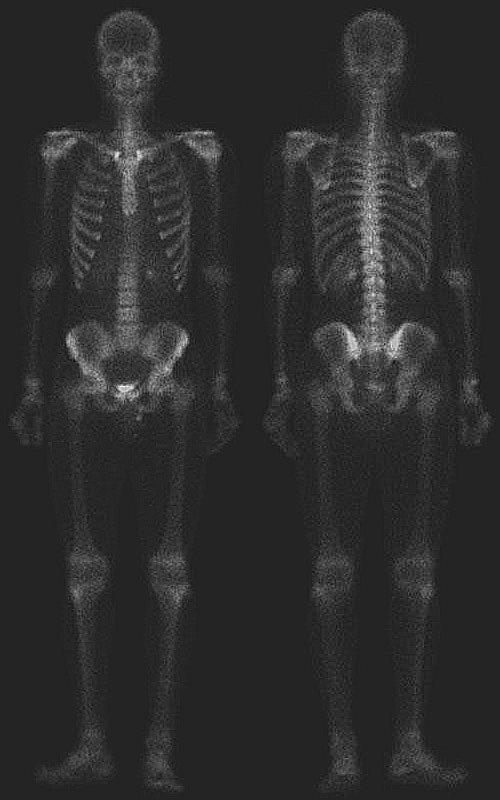
\includegraphics[height=200pt]{./ex2/skeleton_lap_plus_orig.jpg}
	\caption{Sum of laplacian and original image}
\end{figure}
\begin{figure}[!ht]
	\centering
	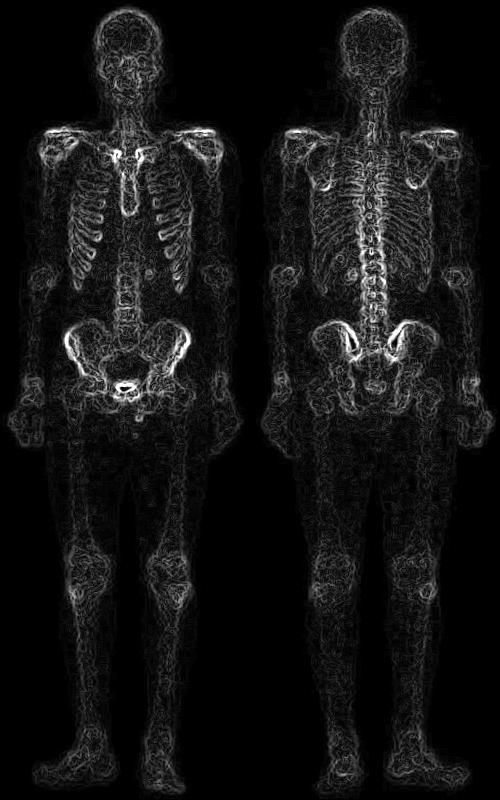
\includegraphics[height=200pt]{./ex2/skeleton_sobel.jpg}
	\caption{Sobel gradient of original image}
\end{figure}
\begin{figure}[!ht]
	\centering
	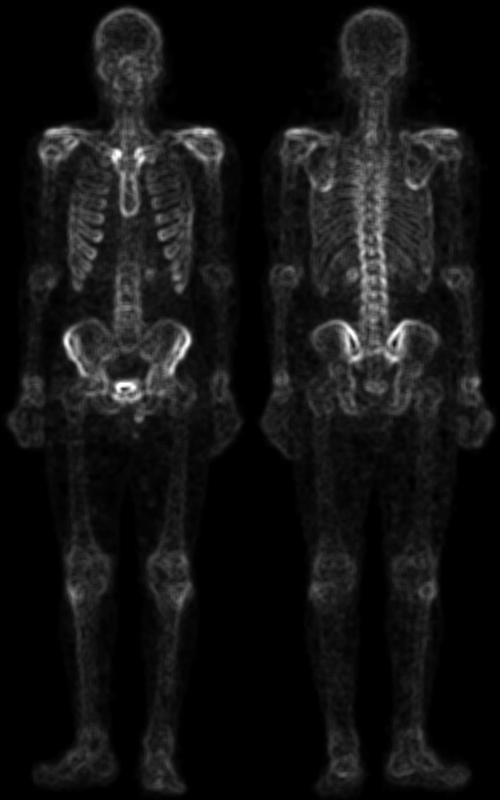
\includegraphics[height=200pt]{./ex2/skeleton_smmoth_sobel.jpg}
	\caption{Smoothed Sobel gradient of original image}
\end{figure}
\begin{figure}[!ht]
	\centering
	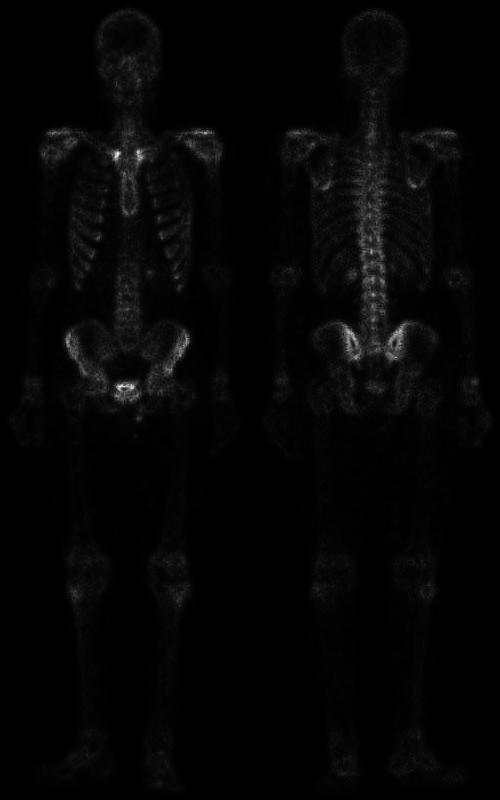
\includegraphics[height=200pt]{./ex2/skeleton_product.jpg}
	\caption{Product of smoothed Sobel gradient and of the previous sum of laplacian and original}
\end{figure}
\begin{figure}[!ht]
	\centering
	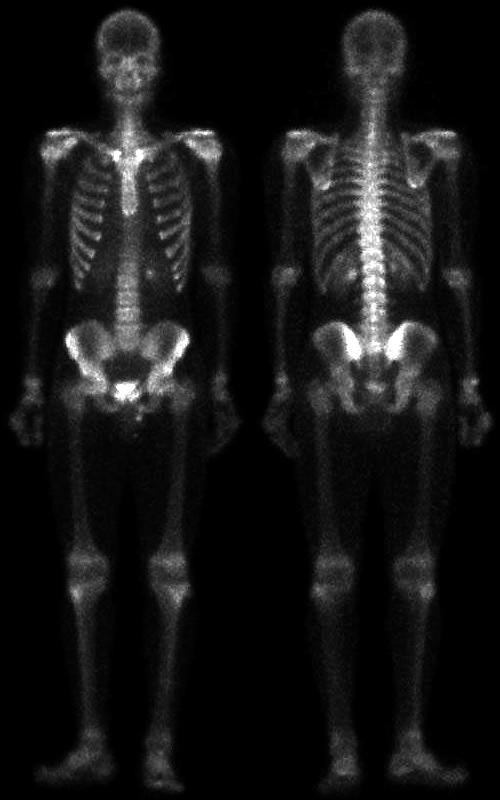
\includegraphics[height=200pt]{./ex2/skeleton_final.jpg}
	\caption{Sum of original image and previous image}
\end{figure}
\begin{figure}[!ht]
	\centering
	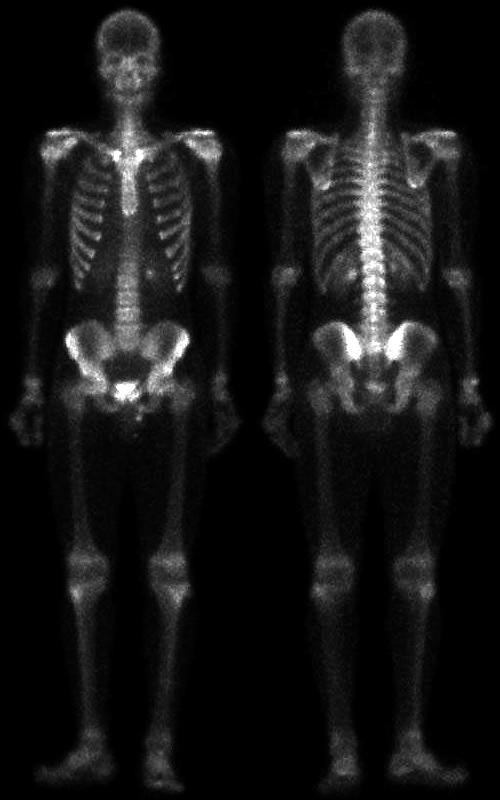
\includegraphics[height=200pt]{./ex2/skeleton_final.jpg}
	\caption{Power law of original image, gamma = 0.5, c = 1}
\end{figure}

\clearpage

\section{Exercise 3}
The program called ex3.py performs several frequency domain enhancement techniques on a given greyscale image.
\subsection{Examples}
\subsubsection{Ideal filter}
Those images are obtained using the call "./ex3 --ideal --highpass cutoff image" for highpass images, and "./ex3 --ideal --lowpass cutoff image" for lowpass images.
\begin{figure}[!ht]
	\centering
	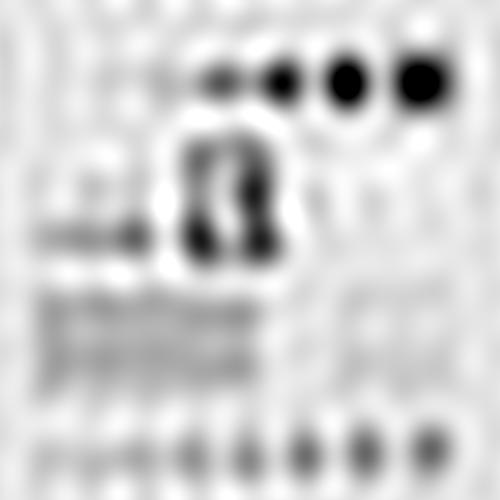
\includegraphics[height=200pt]{./ex3/ch_ideal_low_10.jpg}
	\caption{Cutoff 10 Ideal lowpass filter}
\end{figure}
\begin{figure}[!ht]
	\centering
	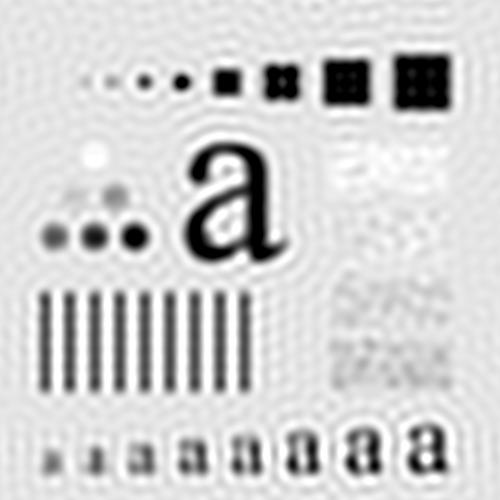
\includegraphics[height=200pt]{./ex3/ch_ideal_low_30.jpg}
	\caption{Cutoff 30 Ideal lowpass filter}
\end{figure}
\begin{figure}[!ht]
	\centering
	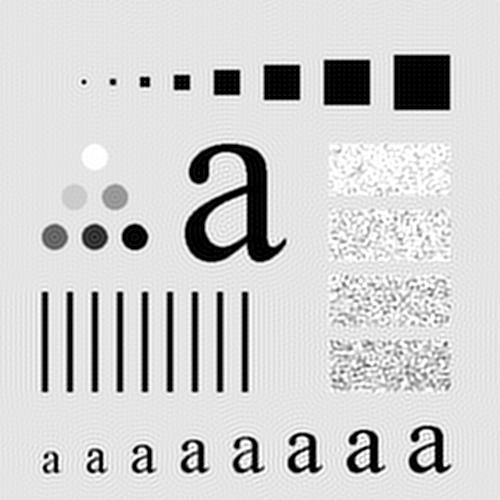
\includegraphics[height=200pt]{./ex3/ch_ideal_low_100.jpg}
	\caption{Cutoff 100 Ideal lowpass filter}
\end{figure}
\begin{figure}[!ht]
	\centering
	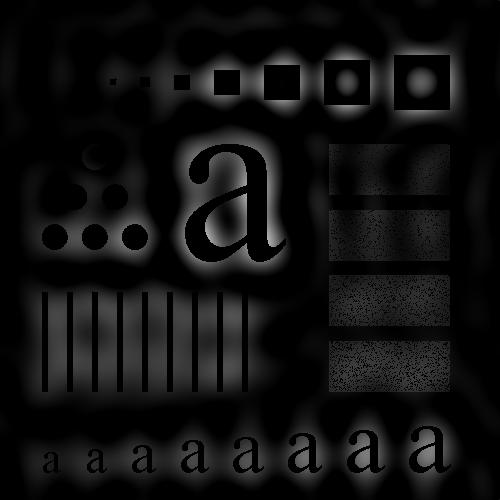
\includegraphics[height=200pt]{./ex3/ch_ideal_high_10.jpg}
	\caption{Cutoff 10 Ideal highpass filter}
\end{figure}
\begin{figure}[!ht]
	\centering
	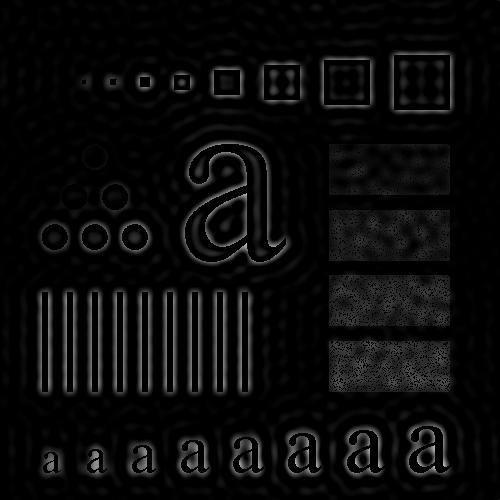
\includegraphics[height=200pt]{./ex3/ch_ideal_high_30.jpg}
	\caption{Cutoff 30 Ideal highpass filter}
\end{figure}
\begin{figure}[!ht]
	\centering
	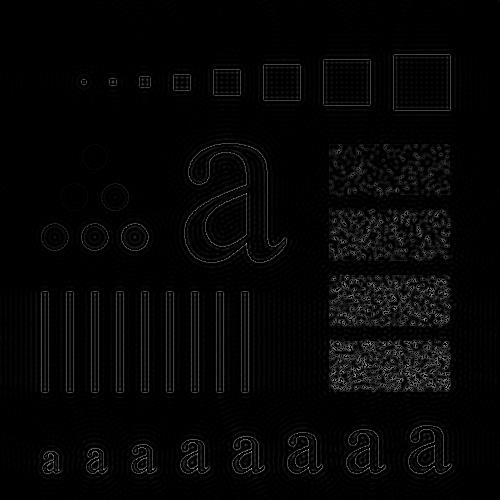
\includegraphics[height=200pt]{./ex3/ch_ideal_high_100.jpg}
	\caption{Cutoff 100 Ideal highpass filter}
\end{figure}
\clearpage
\subsubsection{Gaussian filter}
Those images are obtained using the call "./ex3 --gaussian --highpass cutoff image" for highpass images, and "./ex3 --gaussian --lowpass cutoff image" for lowpass images.
\begin{figure}[!ht]
	\centering
	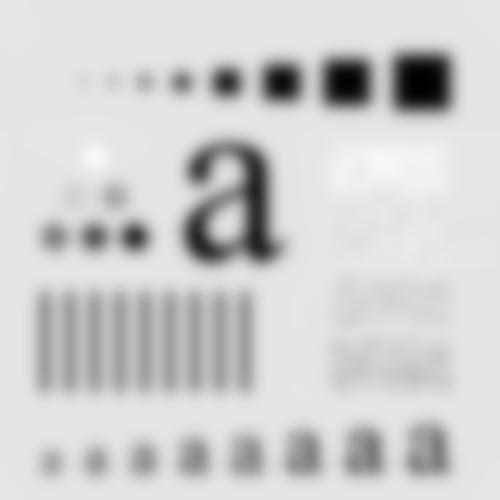
\includegraphics[height=200pt]{./ex3/ch_gauss_low_10.jpg}
	\caption{Cutoff 10 Gaussian lowpass filter}
\end{figure}
\begin{figure}[!ht]
	\centering
	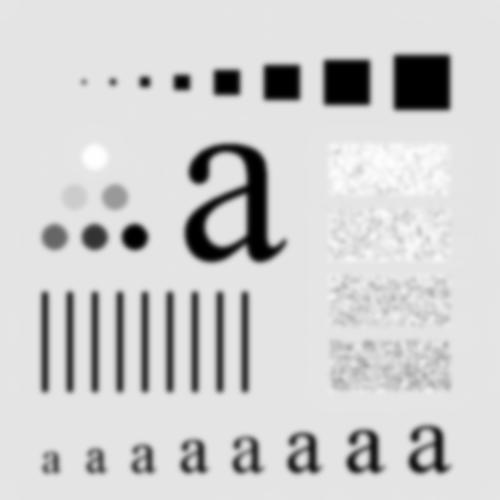
\includegraphics[height=200pt]{./ex3/ch_gauss_low_30.jpg}
	\caption{Cutoff 30 Gaussian lowpass filter}
\end{figure}
\begin{figure}[!ht]
	\centering
	
\includegraphics[height=200pt]{./ex3/ch_gauss_low_100.jpg}
	\caption{Cutoff 100 Gaussian lowpass filter}
\end{figure}
\begin{figure}[!ht]
	\centering
	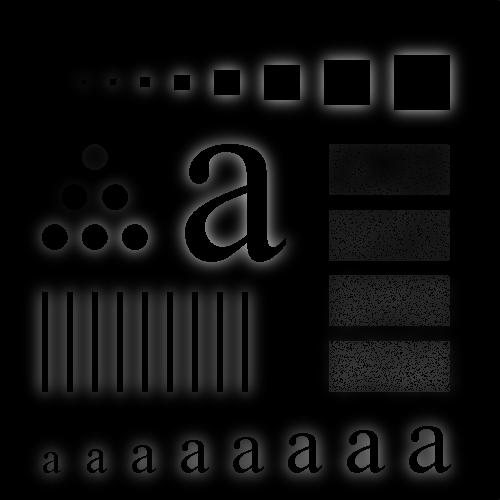
\includegraphics[height=200pt]{./ex3/ch_gauss_high_10.jpg}
	\caption{Cutoff 10 Gaussian highpass filter}
\end{figure}
\begin{figure}[!ht]
	\centering
	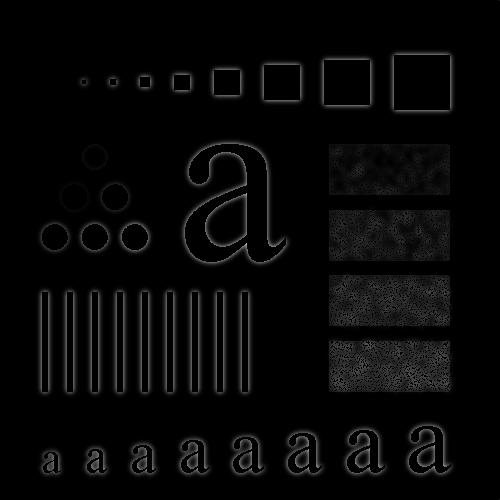
\includegraphics[height=200pt]{./ex3/ch_gauss_high_30.jpg}
	\caption{Cutoff 30 gaussian highpass filter}
\end{figure}
\begin{figure}[!ht]
	\centering
	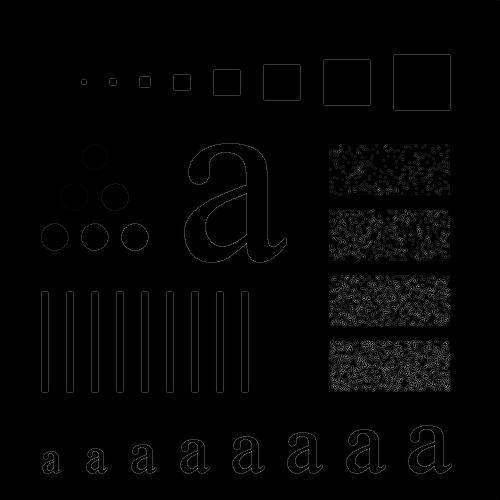
\includegraphics[height=200pt]{./ex3/ch_gauss_high_100.jpg}
	\caption{Cutoff 100 Gaussian highpass filter}
\end{figure}
\clearpage
\subsubsection{Butterworth filter}
Those images are obtained using the call "./ex3 --butterworth --highpass --order order cutoff image" for highpass images, and "./ex3 --butterworth --lowpass --order order cutoff image" for lowpass images.
\begin{figure}[!ht]
	\centering
	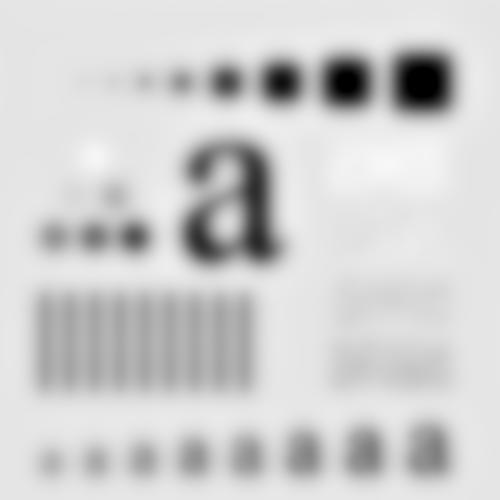
\includegraphics[height=200pt]{./ex3/ch_butter_low_10.jpg}
	\caption{Cutoff 10 order 2 Butterworth lowpass filter}
\end{figure}
\begin{figure}[!ht]
	\centering
	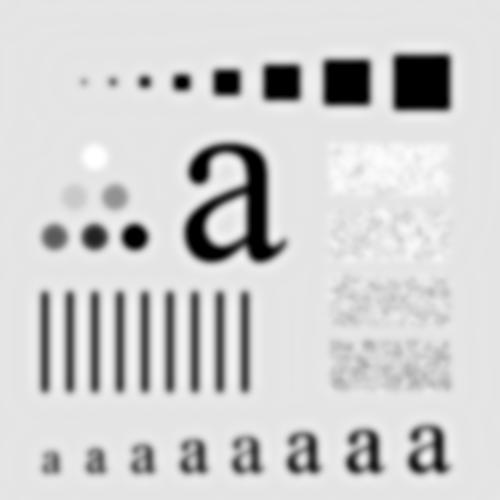
\includegraphics[height=200pt]{./ex3/ch_butter_low_30.jpg}
	\caption{Cutoff 30 order 2 Butterworth lowpass filter}
\end{figure}

\begin{figure}[!ht]
	\centering
	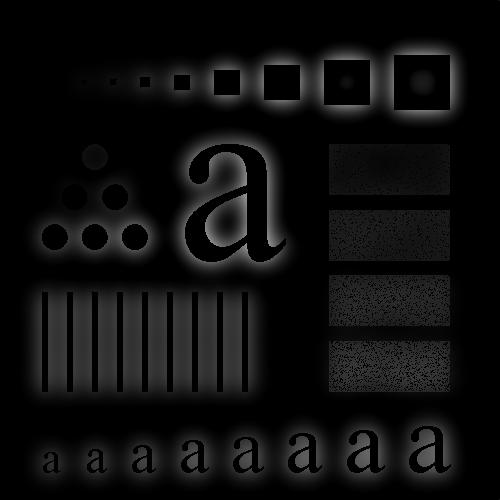
\includegraphics[height=200pt]{./ex3/ch_butter_high_10.jpg}
	\caption{Cutoff 10 order 2 Butterworth highpass filter}
\end{figure}
\begin{figure}[!ht]
	\centering
	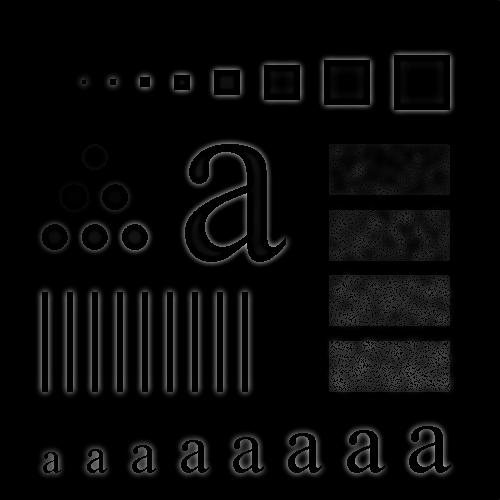
\includegraphics[height=200pt]{./ex3/ch_butter_high_30.jpg}
	\caption{Cutoff 30 order 2 Butterworth highpass filter}
\end{figure}

\clearpage

\section{Exercise 4}
For exercise 4, the program gaussNoise.py adds gaussian noise of desired mean and variance o an image.
The program uniNoise.py adds uniform noise of desired lower and upper bound to an image.
The program filtering.py uses different means of filtering an image.
\subsection{Examples}
\begin{figure}[!ht]
	\centering
	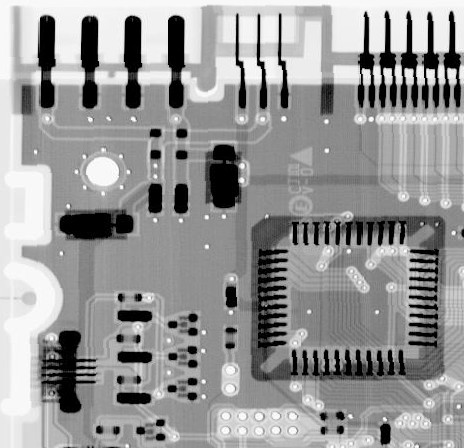
\includegraphics[height=200pt]{./ex4/Circuit.jpg}
	\caption{Original image}
\end{figure}
\begin{figure}[!ht]
	\centering
	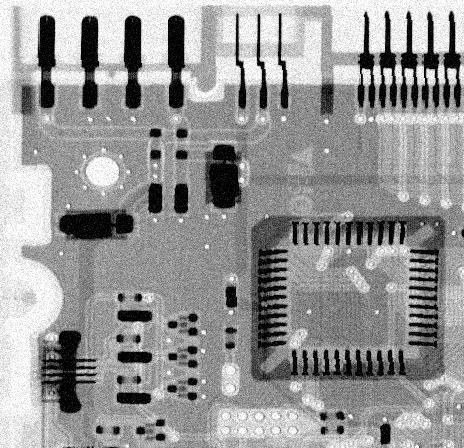
\includegraphics[height=200pt]{./ex4/gaussC.jpg}
	\caption{Original image with gaussian noise of mean 0 and variance 260}
\end{figure}
\begin{figure}[!ht]
	\centering
	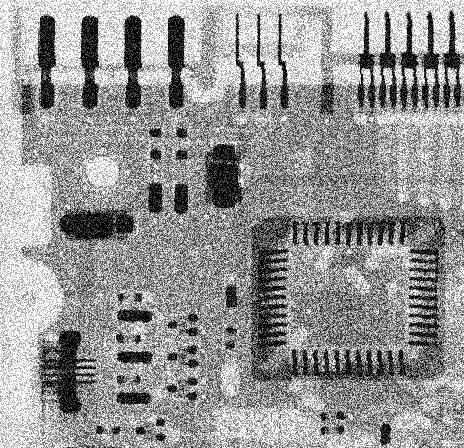
\includegraphics[height=200pt]{./ex4/uniC.jpg}
	\caption{Original image with uniform noise in the [-100, 100] range}
\end{figure}
\begin{figure}[!ht]
	\centering
	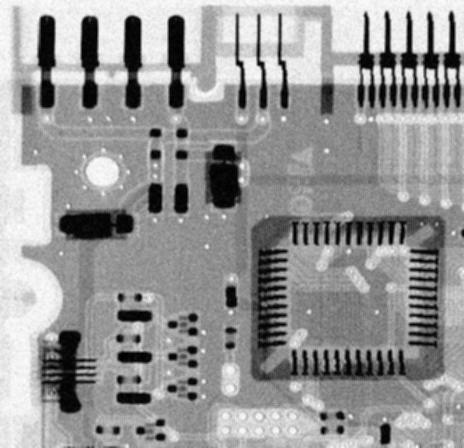
\includegraphics[height=200pt]{./ex4/gaussarith.jpg}
	\caption{Image with gaussian noise enhanced with arithmetic mean}
\end{figure}
\begin{figure}[!ht]
	\centering
	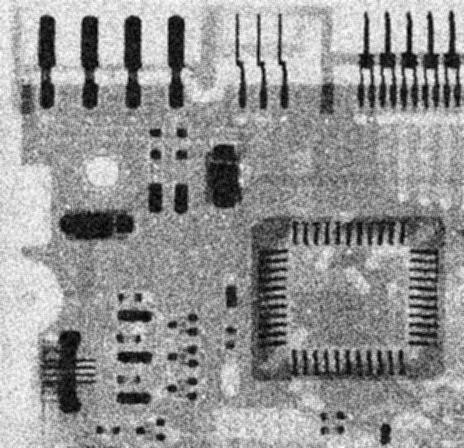
\includegraphics[height=200pt]{./ex4/uniarith.jpg}
	\caption{Image with uniform noise enhanced with arithmetic mean}
\end{figure}

\begin{figure}[!ht]
	\centering
	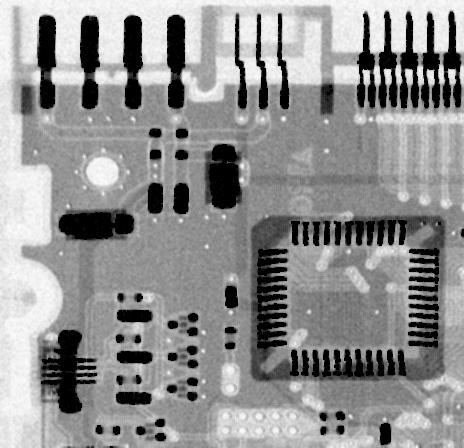
\includegraphics[height=200pt]{./ex4/gaussgeo.jpg}
	\caption{Image with gaussian noise enhanced with geometric mean}
\end{figure}
\begin{figure}[!ht]
	\centering
	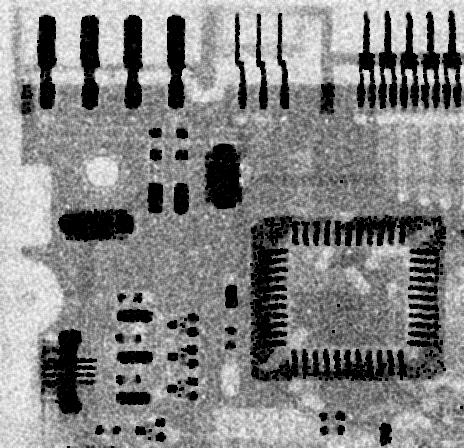
\includegraphics[height=200pt]{./ex4/unigeo.jpg}
	\caption{Image with uniform noise enhanced with geometric mean}
\end{figure}

\begin{figure}[!ht]
	\centering
	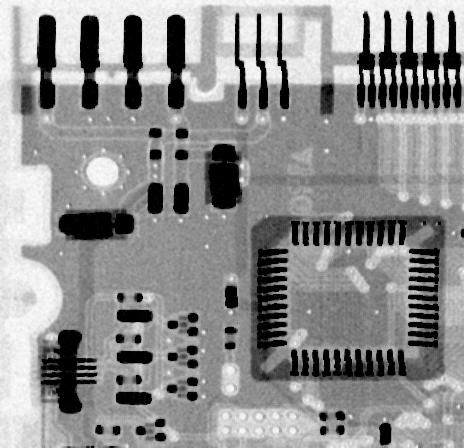
\includegraphics[height=200pt]{./ex4/gaussharmo.jpg}
	\caption{Image with gaussian noise enhanced with harmonic filter}
\end{figure}
\begin{figure}[!ht]
	\centering
	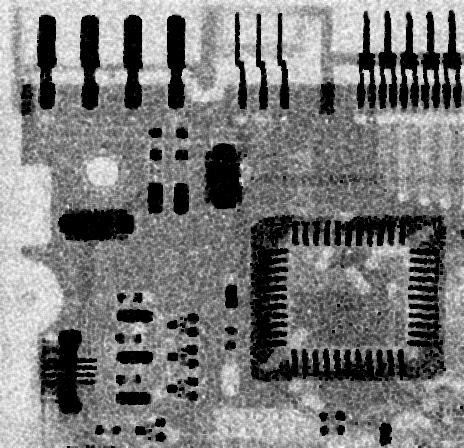
\includegraphics[height=200pt]{./ex4/uniharmo.jpg}
	\caption{Image with uniform noise enhanced with harmonic filter}
\end{figure}

\begin{figure}[!ht]
	\centering
	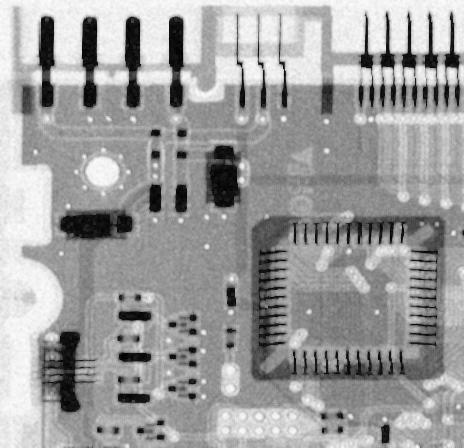
\includegraphics[height=200pt]{./ex4/gaussch15.jpg}
	\caption{Image with gaussian noise enhanced with contra harmonic filter of order 1.5}
\end{figure}
\begin{figure}[!ht]
	\centering
	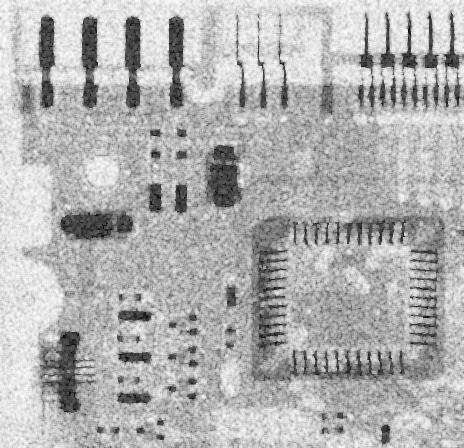
\includegraphics[height=200pt]{./ex4/unich15.jpg}
	\caption{Image with uniform noise enhanced with contra harmonic filter of order 1.5}
\end{figure}

\begin{figure}[!ht]
	\centering
	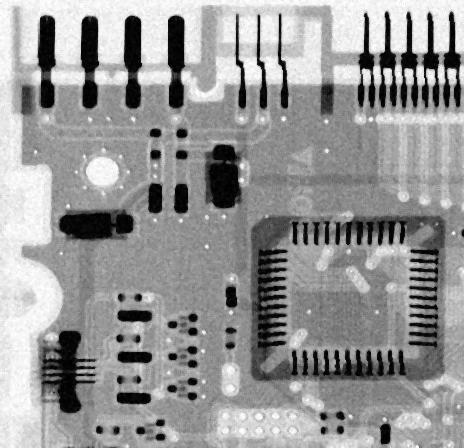
\includegraphics[height=200pt]{./ex4/gaussmedian.jpg}
	\caption{Image with gaussian noise enhanced with median filter}
\end{figure}
\begin{figure}[!ht]
	\centering
	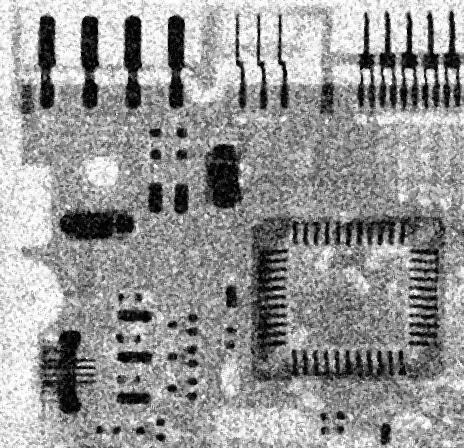
\includegraphics[height=200pt]{./ex4/unimedian.jpg}
	\caption{Image with uniform noise enhanced with median filter}
\end{figure}

\begin{figure}[!ht]
	\centering
	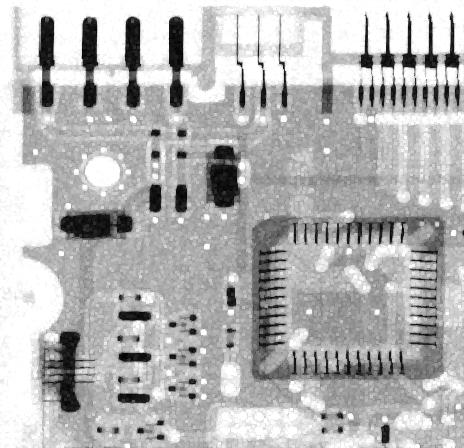
\includegraphics[height=200pt]{./ex4/gaussmax.jpg}
	\caption{Image with gaussian noise enhanced with max filter}
\end{figure}
\begin{figure}[!ht]
	\centering
	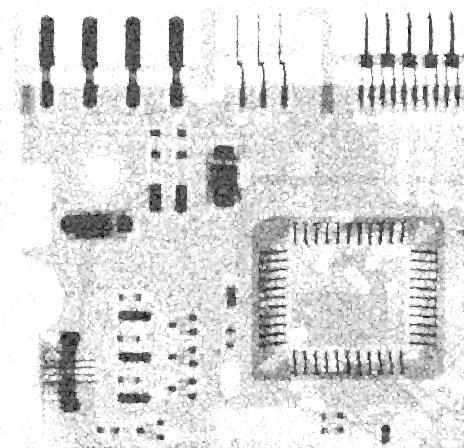
\includegraphics[height=200pt]{./ex4/unimax.jpg}
	\caption{Image with uniform noise enhanced with max filter}
\end{figure}

\begin{figure}[!ht]
	\centering
	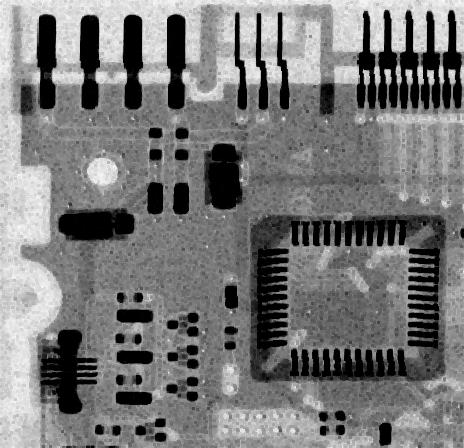
\includegraphics[height=200pt]{./ex4/gaussmin.jpg}
	\caption{Image with gaussian noise enhanced with min filter}
\end{figure}
\begin{figure}[!ht]
	\centering
	\includegraphics[height=200pt]{./ex4/unimin.jpg}
	\caption{Image with uniform noise enhanced with min filter}
\end{figure}

\clearpage
\begin{figure}[!ht]
	\centering
	\includegraphics[height=200pt]{./ex4/gaussmid.jpg}
	\caption{Image with gaussian noise enhanced with midpoint filter}
\end{figure}
\begin{figure}[!ht]
	\centering
	\includegraphics[height=200pt]{./ex4/unimid.jpg}
	\caption{Image with uniform noise enhanced with midpoint filter}
\end{figure}

\begin{figure}[!ht]
	\centering
	\includegraphics[height=200pt]{./ex4/gaussalpha2.jpg}
	\caption{Image with gaussian noise enhanced with alpha trimmed filter of order 2}
\end{figure}
\begin{figure}[!ht]
	\centering
	\includegraphics[height=200pt]{./ex4/unialpha2.jpg}
	\caption{Image with uniform noise enhanced with alpha trimmed filter of order 2}
\end{figure}


\clearpage

\end{document}